\documentclass[12pt, fullpage,letterpaper]{article}

\usepackage[margin=1in]{geometry}
\usepackage{url}
\usepackage{amsmath}
\usepackage{float}
\usepackage{graphicx}

\newcommand{\assignmentId}{1}

\newcommand{\bx}{{\bf x}}
\newcommand{\bw}{{\bf w}}



\begin{document}
	\begin{titlepage}
		\centering
		\vspace*{2cm}
		{\scshape\LARGE Data Mining\par}
		\vspace{.2cm}
		{\huge\bfseries Intermediate Report\par}
		\vspace{1cm}
		{\large\itshape Jadon Wagstaff\par}
		{\large\itshape Christian Felt\par}
		\vfill
		{\large March 20, 2017}
	\end{titlepage}
	
	\section{Introduction}
	Data was obtained from the International Union for the Conservation of Nature (IUCN) via shapefiles. The files contained sets of polygons representing the ranges of different species assessed by the IUCN. The problem is: how do we answer the question of ''where are areas of high biodiversity?'' We divided the work into two parts. Christian created centroids of each polygon and implemented clustering algorithms discussed in class. Jadon explored other methods of clustering.
	
	\section{Class Methods}
	Using ArcMap software, I computed the centroids of the polygons that represent the ranges of terrestrial mammal, reptile, and amphibian species in the IUCN shapefiles. Using my own Python code, I turned the latitude and longitude coordinates of these centroids into a 2-dimensional matrix and performed various kinds of clustering, trying to find areas of especially high density of endangered species.
	
	To measure distance, I used the great-circle distance as given by d from the Haversine formula, where $\phi$ latitude, $\lambda$ is longitude, and $R$ is the radius of the earth.
	\begin{equation}
		a = \sin^2 \frac{\Delta\phi}{2} + \cos \phi_1 (\cos \phi_2)  (\sin^2 \frac{\Delta\lambda}{2})
	\end{equation}
	\begin{equation}
		c =  \begin{cases} 
				0 & a = 0 \cr \tan^{-1}{\frac{\sqrt{1-a}}{a}} & a \neq 0
			\end{cases}
	\end{equation}
	\begin{equation}
		d = R*c
	\end{equation}
	
	Since the Earth is not perfectly spherical, the great-circle distance may be wrong by up to approximately 0.3\% or 22km according to the analysis at http://gis.stackexchange.com/q/25494. In their article “Global Patterns of Terrestrial Vertebrate Diversity and Conservation,” Jenkins et al set 100km as a reasonable lower limit for “fine-grained spatial analysis” in this field.
	
	Hierarchical clustering ran too slowly for the full dataset (74,529 points) or for amphibians alone (18,694 points). K-means++ worked for small numbers of clusters (20 or less) but became obnoxiously slow for larger k. Lloyd’s was also too slow for more than about 20 clusters.
	
	Gonzalez clustering processed the entire dataset in less than 10 seconds. Using the “elbow” principle, I chose k=40 (see Figure 1). The resulting clusters (see Figure 2) seem surprisingly reasonable, often lining up with the “25 Global Biodiversity Hotspots” shown in Figure 3. For instance, Gonzalez gives Madagascar, New Zealand, and the Caucasus Mountains their own clusters, separates the Pacific Northwest from the rest of the Rockies, and divides up the Amazonian, Congo, and Indonesian rainforests in roughly canonical ways. Also, the Aleutian and Canary Islands, Newfoundland, and Hawaii are given their own clusters, and the Andes, Himalayas, and other mountain chains are not too broken up. 
	
	On the other hand, areas with low density of endangered species, such as Siberia or the Sahara Desert, seem to get partitioned in fairly meaningless ways. Also, my clusters assign the Mediterranean Basin, somewhat oddly, to 3 different centers. 
	
	But if my clustering inspires confidence by reflecting the common knowledge in some areas, then perhaps where it deviates from the usual boundaries, the results should not be immediately dismissed. They might provide questions for further research. For instance, is there really a significant difference in the species and habitats of the western half of the Mediterranean Basin versus the half that lies to the east of Sicily? What (if anything) justifies the separation of India from Indochina, Scotland from the rest of the U.K., or the area along the coast of West Africa from the Congo River Basin at a right angle to the south?
	
	\section{Other Methods}
	Since the question is ''where are areas of high biodiversity?'' a density based clustering algorithm is a natural choice. Additionally, a paper on the topic (Joshi, 2011) gives evidence that density based algorithms are good option for solving polygon clustering problems (will be properly cited in final paper). Using the centroid data, the Haversine distance metric, and suggestions from Joshi(2011), an implementation of a modified version of dbscan was created in C++.
	\begin{tabbing}
		Mod\= ifie\= d db\= scan algorithm:\\
		\> Choose distance $\epsilon$ and number of points $minPts$\\
		\> Go to each data point and if it is unlabelled\\
		\> \> If the number of data points within $\epsilon$ is less than $minPts$\\
		\> \> \> label it outlier\\
		\> \> otherwise\\
		\> \> \> label it and all nearby core points as part of the same cluster\\
		\> \> \> label all border points of cluster as part of the same cluster\\
	\end{tabbing}

	Run-time for the implementation on all  74,529 centroids was about half an hour. The results are displayed in figure 4. An epsilon radius of 75km seemed to produce good clusters, but more inquiry is required to determine what is an optimal value.
	
	Another topic of conversation in Joshi(2011) is desirable methods of measuring distance between two closed sets (polygons) $A$ and $B$. They show that Hausdorf Distance $H(A,B)$ has desirable qualities and demonstrate its usefulness in their own implementation. The problem we face is that each of the polygons in our dataset are quite complex, so we need to determine if there is a viable implementation method for calculating these distances.
	\begin{equation}
		H(A,B) = \max\left( \left(\max_{a \in A} \left( \min_{b \in B} d(a,b) \right)\right), \left(\max_{b \in B} \left( \min_{a \in A} d(a,b) \right)\right)\right)
	\end{equation}
	
	Here are goals going forward:
	\begin{itemize}
	\item Determine feasibility of implementing Hausdorf distance for dbscan.
	
	\item Implement the modified dbscan on the set of all terrestrial animals using Hausdorf and/or centroids.
	
	\item Query IUCN database to determine which polygons represent species on the red list.
	
	\item Use best implementation method on red list species.
	\end{itemize}
	
	\pagebreak
	
	\begin{figure}[h]
		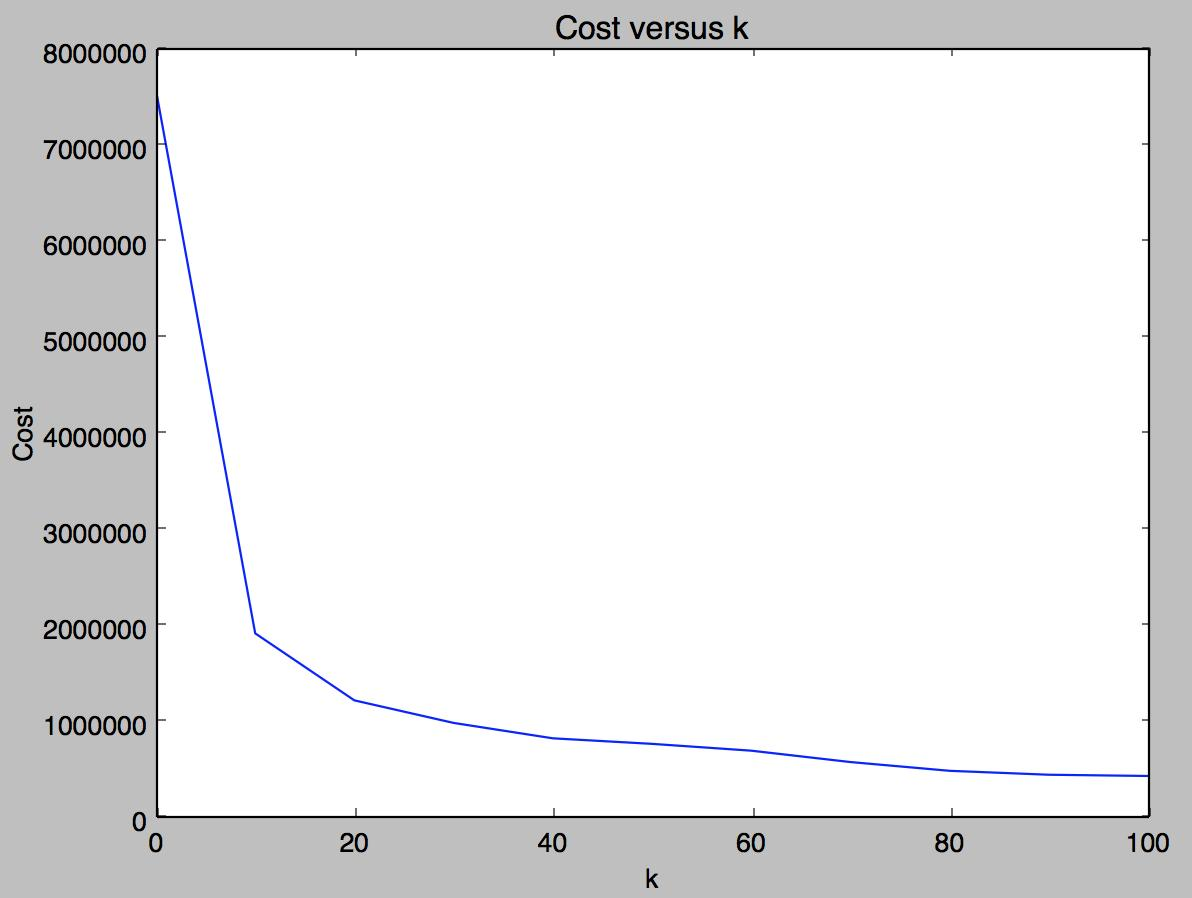
\includegraphics[width=.4\textwidth]{fig1.jpg}
		\caption{Gonzalez analysis}
	\end{figure}
	\begin{figure}[h]
		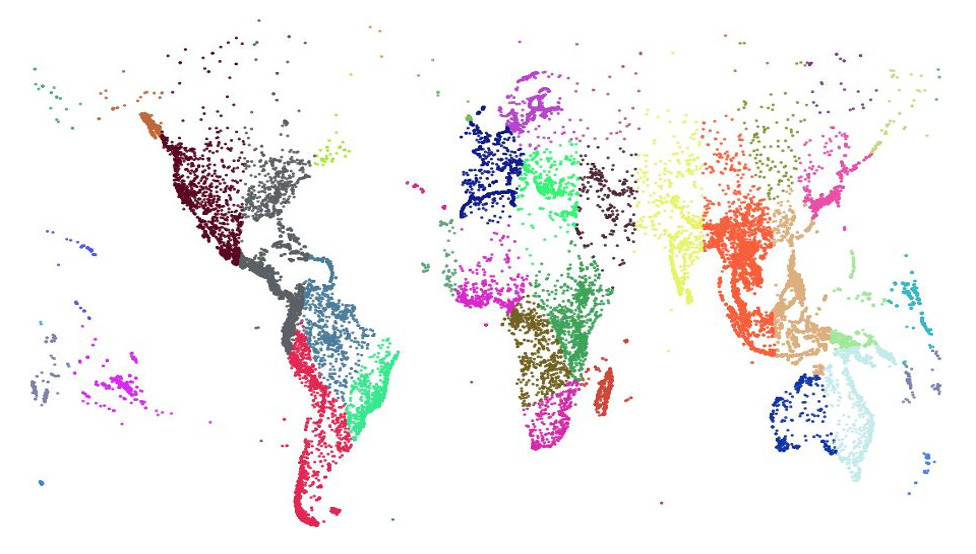
\includegraphics[width=\textwidth]{fig2.jpg}
		\caption{Clustering using Gonzalez}
	\end{figure}
	
	\begin{figure}[h]
		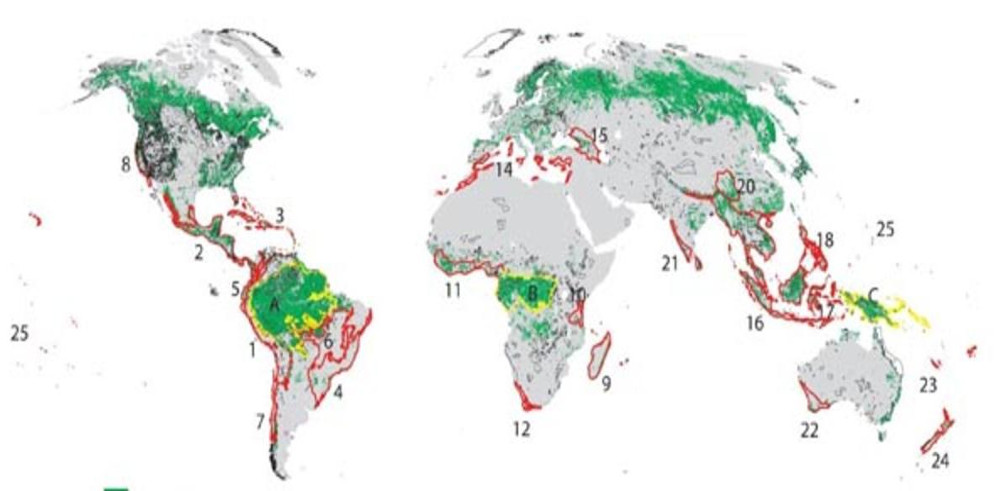
\includegraphics[width=\textwidth]{fig3.jpg}
		\caption{Biodiversity hot-spots}
	\end{figure}
	
	\begin{figure}[h]
		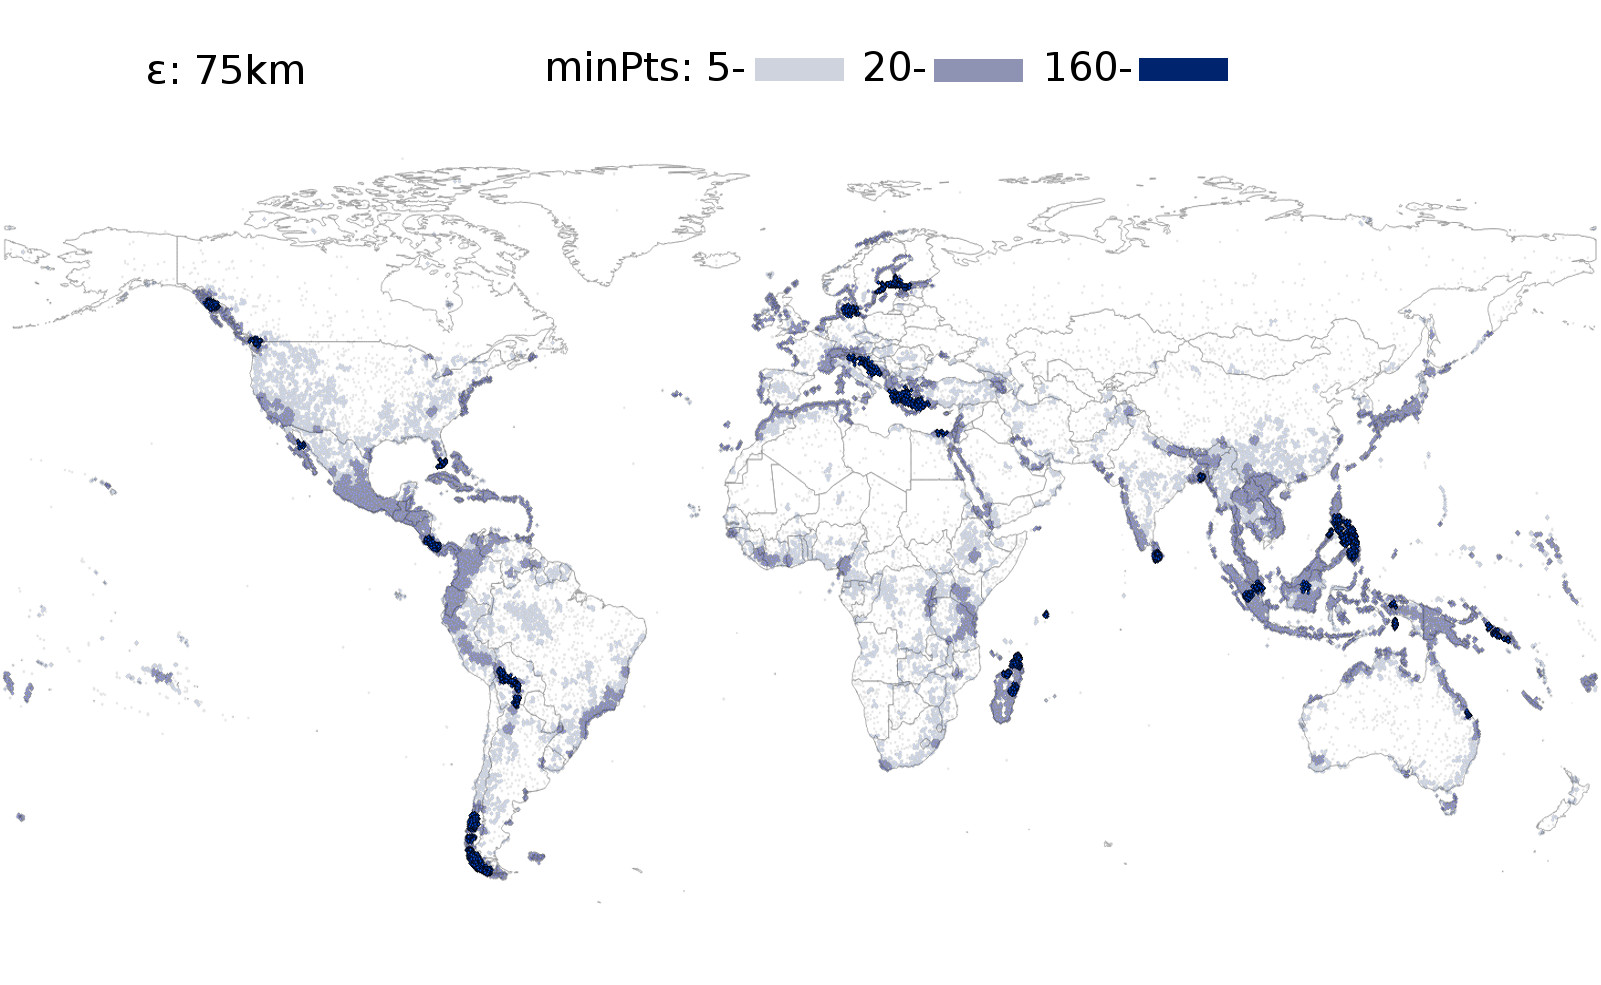
\includegraphics[width=\textwidth]{fig4.jpg}
		\caption{Clustering using dbscan}
	\end{figure}
		
		
	
	
\end{document}